% Figure 3 — one linear-attention layer.
% Standalone: pdflatex fig_layer_tikz.tex -> fig_layer_tikz.pdf.
% txfonts = the fonts elsarticle's `times` option loads, matching the body.
% Same palette tokens as Figure 2 so the two plates read as one system.
\documentclass[border=2pt]{standalone}
\usepackage[T1]{fontenc}
\usepackage{amsmath}
\usepackage{txfonts}
\usepackage{tikz}
\usetikzlibrary{positioning, arrows.meta, calc, fit}

\definecolor{fink}{HTML}{2B3A45}
\definecolor{sandF}{HTML}{F2EFEA}
\definecolor{sandL}{HTML}{7A6F5F}
\definecolor{slate1}{HTML}{E9EEF2}
\definecolor{slate2}{HTML}{D6E0E8}
\definecolor{slateL}{HTML}{4E6371}
\definecolor{brassF}{HTML}{EFDCC6}
\definecolor{brassL}{HTML}{8B6636}
\definecolor{veilF}{HTML}{FBFAF8}

\tikzset{
  dat/.style  = {draw=sandL, fill=sandF, rounded corners=1pt, align=center,
                 font=\footnotesize, inner sep=2pt, minimum height=6mm},
  proj/.style = {draw=slateL, fill=slate1, rounded corners=1pt, align=center,
                 font=\footnotesize, inner sep=2pt, minimum height=6mm},
  gate/.style = {draw=brassL, fill=brassF, rounded corners=1pt, align=center,
                 font=\footnotesize, inner sep=2pt, minimum height=6mm},
  hub/.style  = {draw=brassL, fill=brassF, circle, align=center,
                 font=\footnotesize, inner sep=1.5pt},
  st/.style   = {draw=fink, fill=fink, text=white, rounded corners=1pt,
                 align=center, font=\footnotesize, inner sep=3pt},
  vec/.style  = {draw=sandL, fill=veilF, inner sep=1pt},
  note/.style = {font=\scriptsize, text=fink!85},
  head/.style = {font=\footnotesize, text=fink!90},
  arr/.style  = {->, >={Stealth[length=1.5mm]}, semithick, fink!85},
  bus/.style  = {semithick, fink!85},
}

\newcommand{\conv}[2]{% #1 name, #2 y
  \node[proj, minimum width=13mm, font=\scriptsize] (cv#1) at (4.30,#2) {conv $k{=}4$};}
\newcommand{\barq}[2]{% #1 name, #2 y
  \foreach \i in {0,...,3}{%
    \draw[very thin, sandL, fill=sandF]
      (5.35,#2-0.22+\i*0.11) rectangle ++(0.22,0.11);}}


\begin{document}
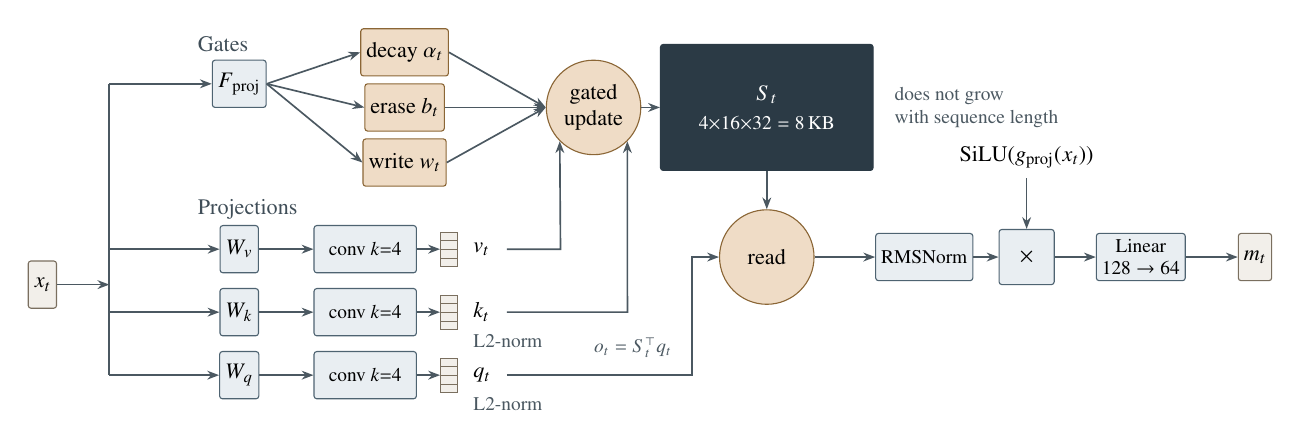
\begin{tikzpicture}

% ---------------------------------------------------------------- input
\node[dat] (xt) at (0.35,4.00) {$x_t$};
\coordinate (split) at (1.20,4.00);
\draw[arr] (xt.east) -- (split);
\draw[bus] (split) -- ++(0,2.55);   % up to the gate row
\draw[bus] (split) -- ++(0,-1.15);  % down to the last projection row

% ---------------------------------------------------------------- gates
\node[head, anchor=west] at (2.20,7.05) {Gates};
\node[proj] (fproj) at (2.85,6.55) {$F_{\text{proj}}$};
\draw[arr] (split |- fproj.west) -- (fproj.west);

\node[gate] (decay) at (4.95,6.95) {decay $\alpha_t$};
\node[gate] (erase) at (4.95,6.25) {erase $b_t$};
\node[gate] (write) at (4.95,5.55) {write $w_t$};
\foreach \g in {decay,erase,write}{\draw[arr] (fproj.east) -- (\g.west);}

\node[hub, minimum size=12mm] (upd) at (7.35,6.25) {gated\\update};
\foreach \g in {decay,erase,write}{\draw[arr] (\g.east) -- (upd.west);}

% ---------------------------------------------------------- projections
\node[head, anchor=west] at (2.20,4.95) {Projections};
\foreach \n/\y in {v/4.45, k/3.65, q/2.85}{
  \node[proj] (w\n) at (2.85,\y) {$W_{\n}$};
  \node[proj, minimum width=13mm, font=\scriptsize] (cv\n) at (4.45,\y) {conv $k{=}4$};
  \foreach \i in {0,...,3}{%
    \draw[very thin, sandL, fill=sandF]
      (5.40,\y-0.22+\i*0.11) rectangle ++(0.22,0.11);}
  \node[font=\footnotesize, anchor=west] at (5.70,\y) {$\n_t$};
  \draw[arr] (split |- w\n.west) -- (w\n.west);
  \draw[arr] (w\n.east) -- (cv\n.west);
  \draw[arr] (cv\n.east) -- (5.40,\y);
}
\node[note, anchor=west] at (5.70,3.28) {L2-norm};
\node[note, anchor=west] at (5.70,2.48) {L2-norm};

% -------------------------------------------------------------- the state
\node[st, minimum width=27mm, minimum height=16mm] (st) at (9.55,6.25)
     {$S_t$\\[1pt]\scriptsize $4{\times}16{\times}32 = 8$\,KB};
\draw[arr] (upd.east) -- (st.west);
\node[note, anchor=west, align=left] at (11.05,6.25)
     {does not grow\\with sequence length};

% ------------------------------------------- k and v write into the state
\draw[arr] (6.25,4.45) -- (6.93,4.45) -- (upd.225);
\draw[arr] (6.25,3.65) -- (7.78,3.65) -- (upd.315);

% ---------------------------------------------------------------- readout
\node[hub, minimum size=12mm] (read) at (9.55,4.35) {read};
\draw[arr] (st.south) -- (read.north);
\draw[arr] (5.70+0.55,2.85) -- (8.60,2.85) -- (8.60,4.35) -- (read.west);
\node[note, anchor=south] at (7.85,2.95) {$o_t = S_t^{\top} q_t$};

\node[proj, font=\scriptsize] (norm) at (11.55,4.35) {RMSNorm};
\node[proj, minimum size=7mm] (mul) at (12.85,4.35) {$\times$};
\node[proj, font=\scriptsize, align=center] (lin) at (14.30,4.35) {Linear\\$128\to64$};
\node[dat] (mt) at (15.75,4.35) {$m_t$};
\draw[arr] (read.east) -- (norm.west);
\draw[arr] (norm.east) -- (mul.west);
\draw[arr] (mul.east) -- (lin.west);
\draw[arr] (lin.east) -- (mt.west);

\node[font=\footnotesize, anchor=south] (silu) at (12.85,5.35)
     {$\mathrm{SiLU}(g_{\text{proj}}(x_t))$};
\draw[arr] (silu) -- (mul.north);

\end{tikzpicture}
\end{document}
